\pagebreak
\subsection{Software Design}

\subsubsection{Purpose}

The purpose of the on-board software consists of:
\begin{itemize}
	\item Controlling the tracking and choosing of targets to observe.
	\item Ensuring that the camera is not oriented towards the sun.
	\item Process and store images taken by camera.
	\item Log housekeeping data.
	\item When possible, send images and housekeeping data to ground station.
\end{itemize}



\subsubsection{Design} \label{sec:4.8.2}

\paragraph{a)} Process Overview\\



\paragraph{b)} General and safety related concepts\\

To ensure that the software is not erroneous rigorous testing will be done during development and after completion. A watchdog timer will be used to avoid software freezing. This timer will reset the on-board computer if it is not itself reset by the software within a certain period. In the case of a reset, the camera shall move to the launch position and tracking restarted.

\paragraph{c)} Interfaces\\



\paragraph{d)} Data acquisition and storage\\

The main bulk of data handled is the images taken by the camera. Housekeeping data such as positioning, camera direction, time, etc will also be stored along with the images.

%need amount of data

%something about cutting out blue & green data ?

\paragraph{e)} Process Flow\\

Pre-launch tests shall be conducted to ensure that all systems work as expected. Afterwards the system shall enter a sleep mode with the camera in a safe launch position. When the float phase is reached, the system will wake. After wake-up the system shall find its orientation and the position of the sun. Finally tracking and observation can start.

Astronomical targets are prioritised. The software shall track and observe the highest priority target within the field of view with varying camera settings until one of the following events happen:

\begin{itemize}
	\item Current target leaves operational field of view.
	\item Target moves too close to the sun for observation.
	\item A higher priority target enters the field of view.
\end{itemize}

If one of the aforementioned events happen, the software will switch current target following prioritisation. While observing targets, the on-board software shall store images and housekeeping data. If connection to ground is available this data shall be compressed using a lossless compression method and sent to ground.

At the end of the floating phase the camera shall be oriented in a landing position and the system shall shut down. Figure \ref{fig:4-8-2-activity-diagram} shows the complete process flow.

\begin{figure}[H] %TODO :figure numbering
    \centering
    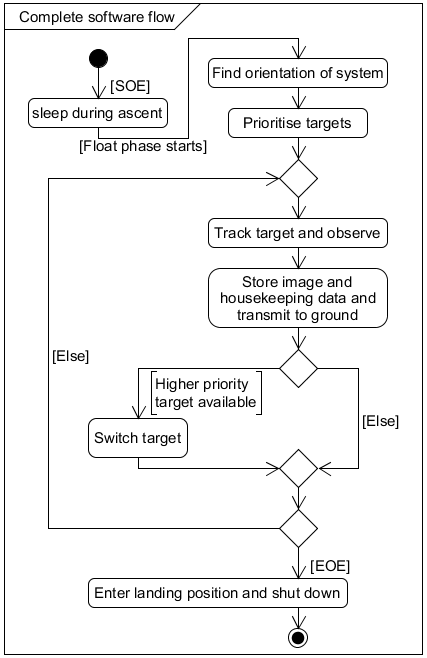
\includegraphics[width=.5\textwidth]{4-experiment-design/img/software/activity-diagram.png}
    \caption{Activity diagram describing the complete software flow.}
    \label{fig:4-8-2-activity-diagram}
\end{figure}


\paragraph{f)} Modularisation and pseudo code\\


\subsubsection{Implementation}\label{sec:4.8.3}

The code for the on-board software shall be implemented in C. An operating system will be used to enable the modularisation required.

\raggedbottom
